% \chapter{Entorno de trabajo y experimentación}
%     \section{Elección del modelo de LLM e hiperparámetros óptimos}
%         \subsection{Modelo de LLM}
%             Elección de GPT-4.
%         \subsection{Hiperparámetros}
%             Temperatura, top\_p, ventana de contexto, número de tokens, etc.
%     \section{Entorno de trabajo}
%         Distinguir entre el entorno de pruebas en chatGPT y el entorno delimitado de la API de OpenAI.
%         \subsection{Entorno de pruebas con chatbot}
%             Útil para experimentación libre. Pero no hay control de los hiperparámetros, las especificaciones pueden cambiar, lo que compromete la repibilidad de los resultados. No permite prompts en 2-steps.
%         \subsection{Entorno de trabajo con la API en Playground y en Python}
%             Hablar de LangChain y de la API de OpenAI.

% \chapter{Estrategias de \textit{prompting} para el diseño sonoro}
%     \section{\textit{Chain of Thoughts} y \textit{Structured Chain of Thoughts}}
%     \section{\textit{1-step} o \textit{2-step}}
%     \section{Uso de \textit{Self-debugging} y \textit{Chain of Verification}}

% \chapter{\textit{System Prompts} y \textit{User Prompts} diseñados para esta investigación}
%     \section{Diseños de \textit{System Prompts}}
%         Han de ser Pocos. Quizás entre 3 y 5. Describir los que se han elegido y lo que se espera de ellos.
%     \section{Diseños de \textit{User Prompts}}
%         Los prompts de usuario escogidos para solicitar al modelo la generación de sonidos y texturas sonoras. Los prompts no deben ser muchos, para poder llevar a cabo la investigación en un tiempo razonable. Deben abarcar diveras técnicas de síntesis, la creación de diversas texturas descritas en lenguaje natural, y la aplicación de teoremas matemáticos, principios físicos, o inspiracion en otras artes, como la pintura o la literatura para la generación sonora.



\chapter{Lenguajes de programación musicales}

Existen en la actualidad numerosos lenguajes de programación musicales, cada uno con sus propias características y orientados a diferentes propósitos. En este capítulo se describen los lenguajes de programación musicales más relevantes, comparando sus características, para finalmente elegir los lenguajes que se utilizarán en esta investigación.

Los lenguajes de programación musicales abarcan tanto la gneración sonora por medio de todo tipo de síntesis, como la manipulación de archivos de audio, la composición musical, la creación de interfaces de usuario, la creación de instalaciones sonoras, la notación musical, etc. No se pretende en este capítulo hacer una descripción exhaustiva de todos los lenguajes de programación musicales existentes, sino más bien una descripción de los lenguajes más relevantes, y que han sido tenidos en cuenta de algún modo en este trabajo. 

\section{Música en código de programación}

Una característica común a los lenguajes de programación musicales es el hecho de que su representación simbólica se realiza por medio de código de programación, en texto plano, y por tanto, son lenguajes formales, con una sintaxis y una semántica definidas. Esto significa que son lenguajes que pueden ser generados por un modelo de lenguaje natural, como los LLM, incluso si no han sido entrenados específicamente en estos lenguajes. Esto es importante, ya que permite que los LLM puedan generar código de estos lenguajes, y por tanto, que puedan generar sonidos y música de un modo indirecto. Los LLM, en su preentrenamiento, han sido entrenados con todo tipo de código, incluyendo lenguajes con propósitos musicales o sonoros. Aunque no podemos esperar que los LLM tengan tanta destreza en Csound como en Python, sí podemos esperar que sean capaces de generar código de Csound, y que este código sea correcto, y que por tanto, pueda ser ejecutado para generar sonidos. Otra cosa es que el código generado sea interesante, o que el sonido generado sea interesante, ni siquiera que el código generado tenga sentido musical. No obstante, explorar esta capacidad de creación musical por medio de la generación de código es uno de los objetivos de esta investigación. La figura \ref{fig:hola_mundo} muestra un \textit{Hola, mundo} en diversos lenguajes de programación sonora, creados todos ellos por medio de GPT-4. Todos ellos tienen en común la generación de un sonido de 440 Hz.

\begin{figure}[h]
    \caption[<<Hola Mundo>> en diferentes lenguajes de programación sonora]{Códigos de <<Hola Mundo>> en diferentes lenguajes de programación sonora. (a) Csound, (b) SuperCollider, (c) Sonic Pi, (d) Overtone (Clojure), (e) FoxDot, (f) ChucK.}
    \centering
    \begin{subfigure}{.48\textwidth}
      \centering
      \begin{mdframed}
      \begin{verbatim}
<CsInstruments>
instr 1
    a1 oscil 0.5, 440, 1
    out a1
endin
</CsInstruments>
<CsScore>
f1 0 1024 10 1
i1 0 2
</CsScore>
      \end{verbatim}
      \end{mdframed}
      \caption{Csound}
    \end{subfigure}\hfill
    \begin{subfigure}{.48\textwidth}
      \centering
      \begin{mdframed}
      \begin{verbatim}
(
SynthDef(\helloworld, {
    Out.ar(0, SinOsc.ar(440, 0, 0.2))
}).add;
)
Synth(\helloworld);

      \end{verbatim}
      \end{mdframed}
      \caption{SuperCollider}
    \end{subfigure}
    
    \vspace{5mm} % Añade espacio vertical entre las filas
    
    \begin{subfigure}{.48\textwidth}
      \centering
      \begin{mdframed}
      \begin{verbatim}
play 72
sleep 1
      \end{verbatim}
      \end{mdframed}
      \caption{Sonic Pi}
    \end{subfigure}\hfill
    \begin{subfigure}{.48\textwidth}
      \centering
      \begin{mdframed}
      \begin{verbatim}
(use 'overtone.live)
(definst hello-world [] (sin-osc 440))
(hello-world)
      \end{verbatim}
      \end{mdframed}
      \caption{Overtone (Clojure)}
    \end{subfigure}
    
    \vspace{5mm} % Espacio vertical entre las filas
    
    \begin{subfigure}{.48\textwidth}
      \centering
      \begin{mdframed}
      \begin{verbatim}
p1 >> pluck([0, 1, 2, 3])
      \end{verbatim}
      \end{mdframed}
      \caption{FoxDot}
    \end{subfigure}\hfill
    \begin{subfigure}{.48\textwidth}
      \centering
      \begin{mdframed}
      \begin{verbatim}
SinOsc s => dac;
440 => s.freq;
1::second => now;
      \end{verbatim}
      \end{mdframed}
      \caption{ChucK}
    \end{subfigure}

    \source{Creado por el autor con GPT-4.}
    \label{fig:hola_mundo}
\end{figure}

Excluimos lenguajes de programación de audio como Pure Data u Open Music, ya que estos lenguajes, si bien guardan sus archivos en formato de texto plano, estos códigos no están diseñados para ser escritos por el usuario, sino sólo como un modo de representación interna de los grafos de objetos que se muestran en un canvas (Figura \ref{fig:patch_puredata}), y que luego son interpretados por un programa de audio. 

\begin{figure}[h]
    \caption[Ejemplo de patch de Pure Data]{Patch de Pure Data en su representación interna en código (a), y en su aspecto visual (b).}
    \centering
    \begin{subfigure}{.48\textwidth}
        \centering
        \begin{mdframed}
        \begin{verbatim}
#N canvas 443 44 725 592 12;
#X declare -stdpath ./;
#X floatatom 127 60 6 0 0 0 - - - 0;
#N canvas 0 0 450 300 (subpatch) 0;
#X array table10 259 float 1;
#X coords 0 1.02 258 -1.02 258 130 1;
#X restore 279 92 graph;
#X text 459 533 updated for Pd version 0.34;
#X text 78 18 WAVETABLE OSCILLATORS;
#X text 25 123 wavetable;
...
        \end{verbatim}
        \end{mdframed}
        \caption{Representación interna en código de un patch de Pure Data}
      \end{subfigure} \hfill

      \vspace{5mm} % Añade espacio vertical entre las filas

      \begin{subfigure}{.48\textwidth}
        \centering
        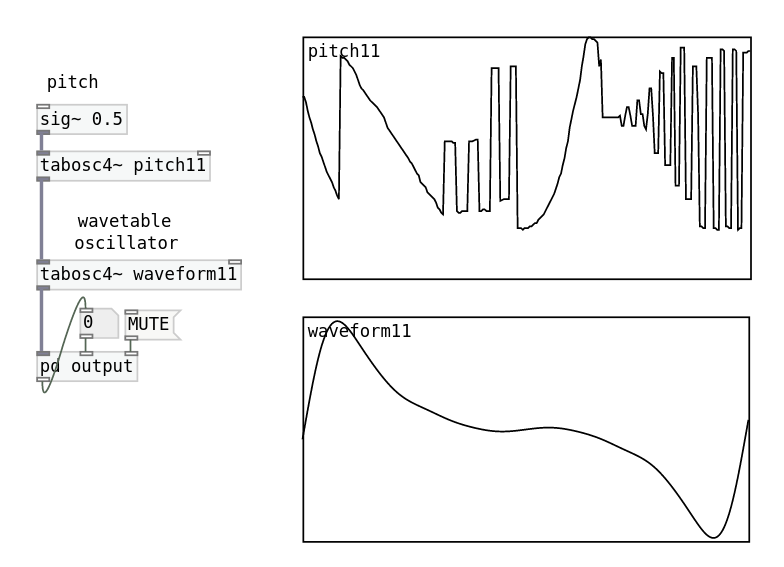
\includegraphics[width=1\textwidth]{./figuras/patch_puredata.png}
        \caption{Aspecto visual de un canvas de Pure Data}
      \end{subfigure}\hfill
    \source{Imagen del autor}
    \label{fig:patch_puredata}
\end{figure}



    
\section{El problema de componer con notas musicales}

Podemos incluir en nuestra lista sistemas de notación musical que se reducen a código, como Lilypond, la librería de Python Music21, ABC notation o el mismo formato MusicXML. Sin embargo, se ha podido comprobar desde un primer acercamiento a LLM como GPT-4, que aún no son capaces de generar un código mínimamente interesante artísticamente cuando hablamos de utilización de notas musicales, acordes, etc., a pesar de comprender perfectamente la sintaxis. La figura \ref{fig:melodia_bach} muestra una partitura generada por GPT-4, cuando se le pidió crear una melodía de 4 compases al estilo de Bach. Como se puede apreciar, la melodía es correcta desde el punto de vista de la sintaxis, pero no tiene ningún interés musical ni atisbo de aproximación estilística al la petición del usuario. Por tanto, se ha decidido excluir de esta investigación los lenguajes de notación musical.

\begin{figure}[h]
    \caption[Melodía de 4 compases generada por GPT-4, al estilo de Bach]{Melodía de 4 compases generada por GPT-4, al estilo de Bach. El LLM la entregó en formato Lilypond.}
    \centering
    \begin{subfigure}{.48\textwidth}
        \centering
        \begin{mdframed}
        \begin{verbatim}
\score {
    \new Staff {
        \key c \major
        \time 4/4
        \tempo 4 = 100
    
        % Compás 1
        c'4 d' e' g' |
    
        % Compás 2
        f' e' d' c' |
    
        % Compás 3
        e'4 f' g' a' |
    
        % Compás 4
        g' f' e' d' |
    }
    \layout { }
    \midi { }
    }
        \end{verbatim}
        \end{mdframed}
        \caption{Código Lilypond devuelto por GPT-4}
      \end{subfigure} \hfill

      \vspace{5mm} % Añade espacio vertical entre las filas

      \begin{subfigure}{.48\textwidth}
        \centering
        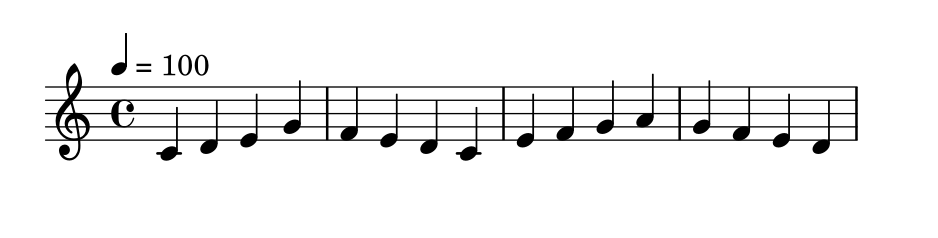
\includegraphics[width=1\textwidth]{./figuras/melodia_bach_estilo.png}
        \caption{Renderizado a notación musical por Lilypond}
      \end{subfigure}\hfill
    \source{Imagen del autor}
    \label{fig:melodia_bach}
\end{figure}

Este mismo problema lo encontramos en cualquier tipo de codificación que utilice notas musicales, como el formato MIDI.
Componer música con notas musicales, con las cotas de complejidad que ha alcanzado la música a lo largo del tiempo y de la geografía, no es una tarea trivial, y va mucho más allá del conocimiento básico de los simbolos utilizados en las diferentes notaciones. La música es un arte, y como tal, requiere de un conocimiento profundo de la teoría musical, de la armonía, del contrapunto, de la historia de la música, de la cultura musical, de la psicología de la percepción musical, etc. Es por ello que no podemos esperar que un LLM sea capaz de generar música con notas musicales de un modo interesante, al menos por el momento.

\section{Lenguajes orientados a la síntesis de sonido}

La música experimental, la música electrónica, la música electroacústica, la música concreta, la música generativa, etc., son géneros musicales que se han desarrollado en el siglo XX, y que han utilizado la tecnología como medio de expresión. En este contexto, han surgido numerosos lenguajes de programación orientados a la síntesis de sonido, que han permitido a los compositores de música electrónica y experimental crear sonidos y música de un modo más flexible y potente que con los sintetizadores analógicos. Estos lenguajes de programación han sido utilizados también en la creación de instalaciones sonoras, en la creación de interfaces de usuario, en la composición musical, etc. 

El lenguaje sonoro en torno a estos géneros musicales es mucho más flexible, por lo general, que el lenguaje de la música notada. Especialmente las músicas autodenominadas experimentales, que no tienen un lenguaje musical definido y que se caracterizan por la búsqueda de nuevos sonidos y nuevas formas de expresión, son idóneas para una experimentación con elementos no humanos, como los LLM. Esta interacción eventualmente puede traducirse en la exploración de nuevos timbres y texturas sonoras.

Dentro de los lenguajes de programación orientados a la síntesis de sonido, podemos distinguir entre los diseñados para ser codificados en interpretaciones en vivo, y los diseñados para ser codificados en archivos de audio, a una composición más estática. \textit{Csound} fue contruido para crear composiciones renderizadas en archivos de audio, si bien actualmente tiene características que le permiten ser ejecutado en tiempo real. \textit{SuperCollider} tiene características de ambos mundos, lo que lo hace óptimo tanto para la composición de obras sonoras como para la codificación en vivo, en lo que se denomina \textit{Live Coding}. Precisamente su ductilidad y potencia lo ha convertido en plataforma de audio sobre la que se han creado otros lenguajes orientados únicamente al tiempo real y \textit{Live Coding}, como \textit{FoxDot}, \textit{Sonic Pi}, \textit{Overtone} o \textit{Tidal Cycles}. Actualmente proliferan lenguajes diseñados para esta interacción en tiempo real con el usuario. Además de los expuestos, podemos destacar \textit{ChucK} o \textit{Strudel}, entre otros. Esto se debe, entre otros factores culturales, al aumento de la potencia de los ordenadores, que permite ejecutar en tiempo real programas de síntesis de sonido cada vez más complejos.